\chapter{Comparative study and analysis}

\section*{Introduction}

\lettrine[lines=2]{A}\\s In order to achieve the objectives of the project, Group 1 researched some of the typical platforms that are currently popular in the industry and analysed their main features, with the aim of incorporating their strengths in the project. Popular software used for the development of digital library systems and platforms include Greenstone, Dspace, Invenio, Omeka S, EPrints, Mukurtu.

\section{Key Features of typical platforms}

\subsection{Greenstone}

Greenstone is basically a relatively complete open source software to meet the needs of the general digital library, but also very suitable for newcomers to start. Its main features are support for multiple languages, multiple digital material formats and cross-platform. greenstone can run on multiple operating systems, including Windows, Mac OS X, Linux, etc. In addition, greenstone supports a variety of open standards and protocols, such as OAI-PMH, Dublin Core, MARC, etc., can Easily integrate digital libraries and web publications with other systems\cite{WelcomeG98:online}.



\subsection{Dspace}

DSpace is an open source digital repository software, the main features of DSpace are its security and community support, DSpace provides a complete permission management system that helps users control who can access and edit the content in the repository while keeping the content secure\cite{DSpaceIn8:online}. 

\begin{figure}[htbp]
  \centerline{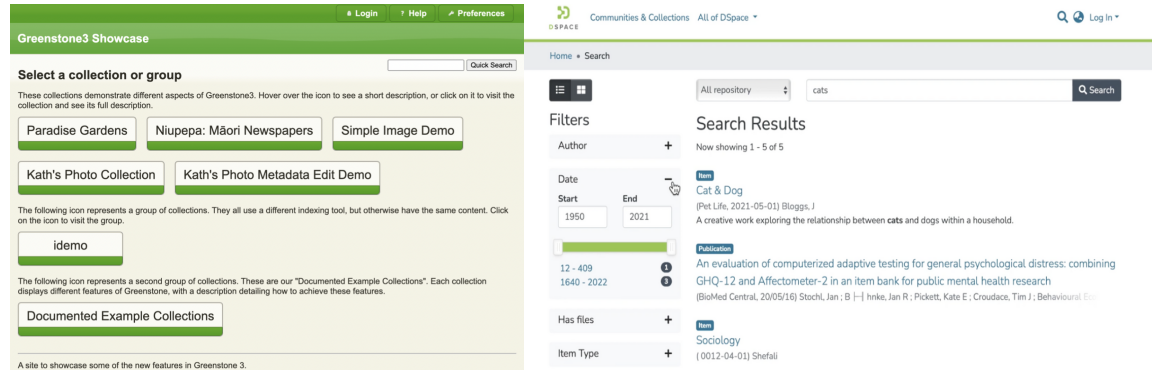
\includegraphics[width=500pt]{images/a1.jpg}}
  \caption{Greenstone \& DSpace}
\end{figure}

\subsection{Invenio}

Invenio is a framework and not a repository software delivered directly. So it requires developers to develop code to refine the implementation of their own platform. Its main features are the powerful search functionality and the ability to handle data storage\cite{Introduc17:online}. It uses all the features of Elasticsearch.



\subsection{Omeka S}
It is a free, open source web application for creating and managing digital documents and online exhibitions.The main feature of Omeka S is the customisable exhibition functionality, with custom exhibition settings based on user needs and support for a wide range of exhibition templates and themes\cite{FeatureL61:online}.

\begin{figure}[htbp]
  \centerline{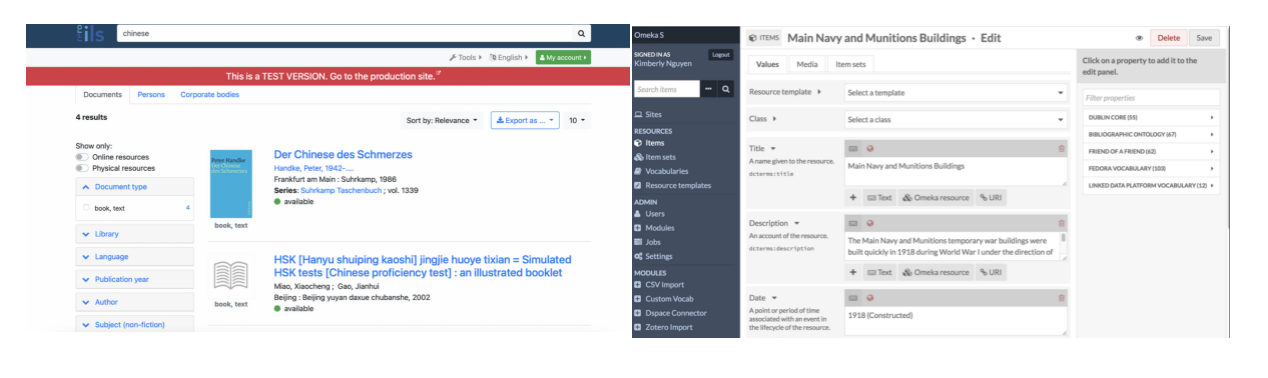
\includegraphics[width=500pt]{images/a9.jpg}}
  \caption{Invenio \& Omeka S}
\end{figure}

\subsection{EPrints}
The main features of EPrints are its support for a wide range of metadata standards and its statistical and analytical functions. It supports a wide range of metadata standards to facilitate the input and output of data. In addition, its statistical and analytical features help users to understand the usage of the digital repository, user preferences for resources, etc\cite{EPrintsS41:online}.


\subsection{Mukurtu}
Mukurtu is an open source digital library and community framework. Its most important feature is that it provides a way of managing cultural heritage that can help preserve and pass on the heritage of a culture. mukurtu's emphasis on community collaboration allows community members to participate in the management and sharing of cultural heritage. In addition, Mukurtu supports the creation and management of cultural protocols, allowing cultural heritage to be managed and shared in accordance with the traditional cultural protocols and norms of the community. This feature allows for the conservation of cultural heritage and the interchange of cultures within the project\cite{AboutMuk17:online}.


\begin{figure}[htbp]
  \centerline{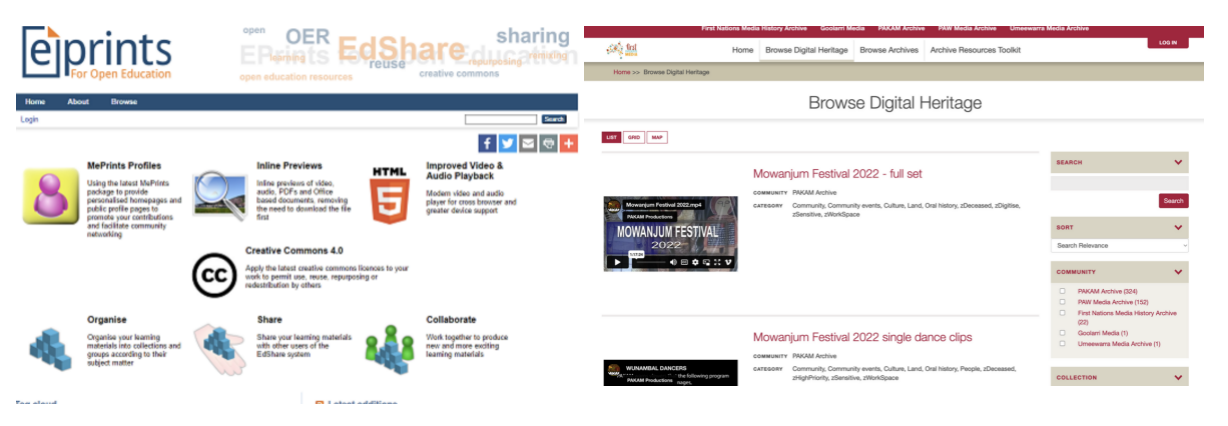
\includegraphics[width=500pt]{images/a8.jpg}}
  \caption{EPrints \& Mukurtu}
\end{figure}


\section{Comparison Chart}
Group 1 has selected a few key attributes that need to be met in a project, comparing the six popular open source software for creating digital libraries mentioned above and creating the following comparison chart. These key attributes can be used to target the advantages of some platforms into our projects.

\begin{figure}[htbp]
  \centerline{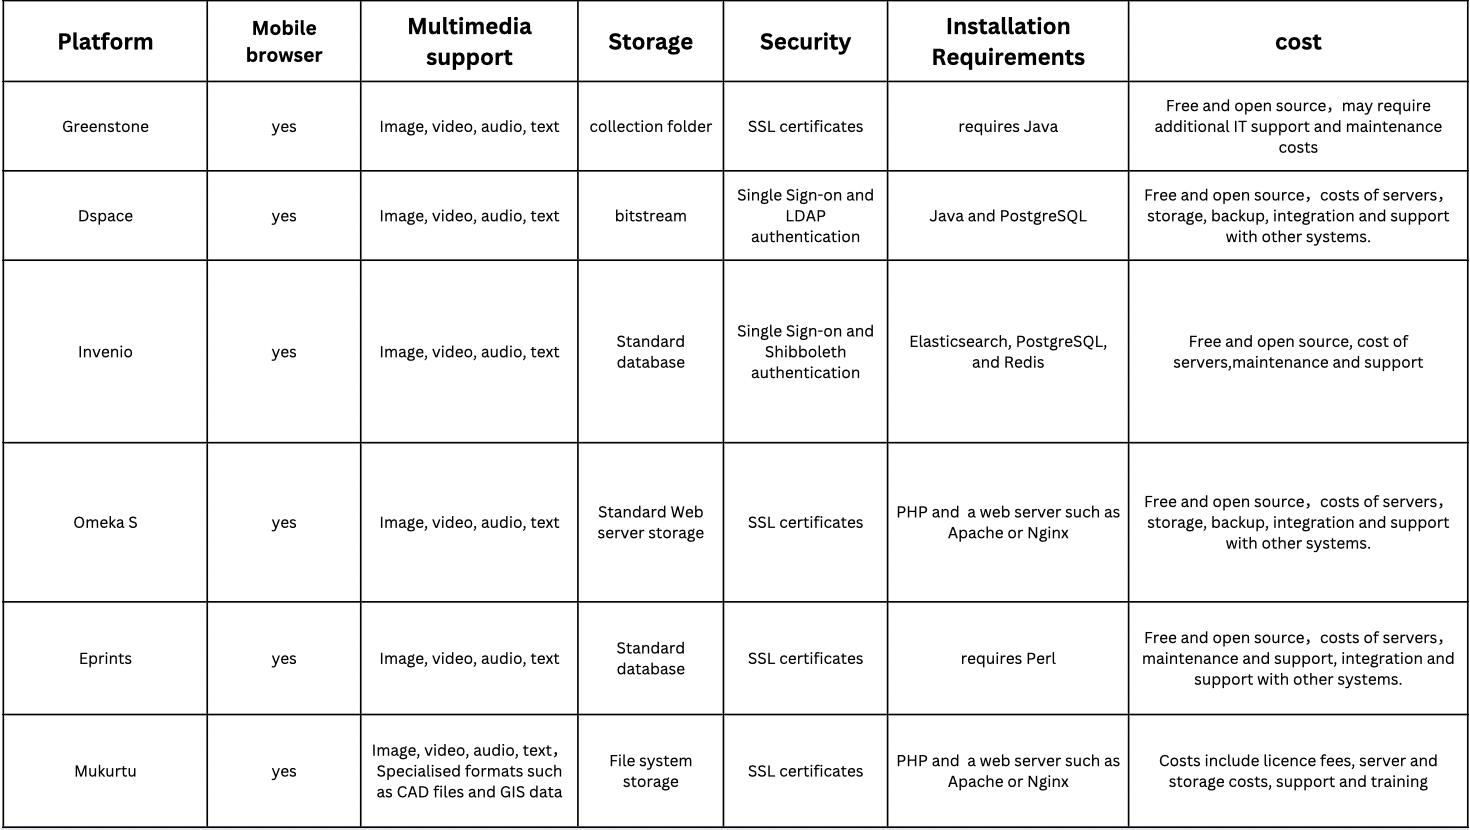
\includegraphics[width=500pt]{images/a2-1.jpg}}
  \caption{Comparison Chart}
\end{figure}


\section{Conclusion}
The main features of six popular open source software for creating digital libraries were analysed through a study of their main features, and according to the requirements of the project, to achieve the transmission and preservation of Māori culture, there was also a need to provide a platform space to allow cultural exchange between members. These requirements are the main aims that need to be achieved. But for the essence of the platform such as data security, multimedia files, cost etc. these are the factors that need to be considered. It is possible to combine the different characteristics of the above platforms and incorporate their main strengths to create the project.

